\section{数値解}
	指数関数と対数関数の交点を、簡単な底の関数で表わすのは難しく見える。そこで、まずは解のグラフを書くことにした。
	グラフを書くために、交点の数値解を数値解析によって求めた。

\subsection{数値解析の方法}
	まずは、不動点解の数値解をニュートン法を用いて求めた。

	ニュートン法とは関数のグラフの傾きを用いて、数値解を求める方法だ。$y=a^x-x$として、適当な$x_0$をとり、
	\[
		x_{n+1} = x_n - \frac{y(x_n)}{y'(x_n)}
	\]
	という漸化式を繰り返し用いていくことで、$y=0$の$x$についての数値解が求められる。
	しかし、ニュートン法では初期値によって求まる解が変わり、また$y'(x_n) \sim 0$であるとき解への収束は不安定になってしまう。
	そこで、$y'(x) = 0$となるような$x$を調べると、$x = -\log_{a} \left(\ln{a}\right)$なので、この値から離れた初期値を採用することで二つの数値解を求めることが出来た。

	次に共役解の数値解を求めた。
	これは$y = a^{x} - \log_{a} x$とすると$y=0$の$x$についての数値解を調べることと同じである。
	しかし、この関数についてニュートン法を適用することは難しい。なぜならば、$y' = a^{x}\ln{a} - \frac{1}{\ln{a}\ln{x}}$が複雑で、初期値を上手く決定できないからだ。

	したがって、二分法を用いてしらみつぶしに調べることにした。

	二分法は、中間値の定理を利用して数値解を求める方法だ。中間値の定理より、$y(m)y(n) < 0$であるような実数$m < n$について、区間$(m,n)$に$y = 0$となる解が存在するといえる。
	さらに、区間$(m,n)$内の実数$l = \frac{m+n}{2}$をとると、$g(m)g(l)$と$g(l)g(n)$の正負を調べることで、区間$(m,l)$と$(l,n)$のどちらに解が存在するかが分かる。
	この分割を十分大きな回数繰り返すと、区間が狭まっていき、最終的には数値解が求められる。

	しかしこの場合、$y$が符号を変えるような区間は事前に分からないという問題がある。そこで、解区間をしらみつぶしに調べることで解決することを考えた。
	共役解が$(0,1)$に存在することは慨形から分かるので、この区間を$2^{10}$程度の小区間に分割し、全てについて二分法を適用することで、共役解を求めることが出来た。

	数値解のグラフを図\ref{fig:all_roots}や図\ref{fig:three_roots}に示す。
	\begin{figure}[hbtp]
	\begin{minipage}{0.5\hsize}
		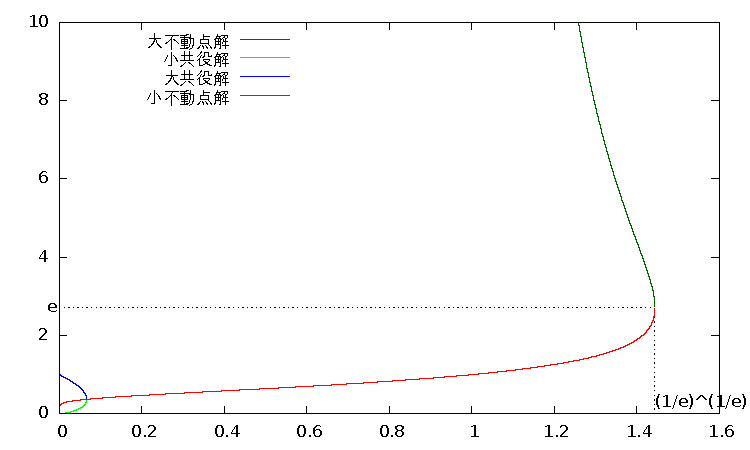
\includegraphics[width=80mm]{../plot/graph/all_roots.pdf}
		\caption{全ての解}
		\label{fig:all_roots}
	\end{minipage}
	\begin{minipage}{0.5\hsize}
		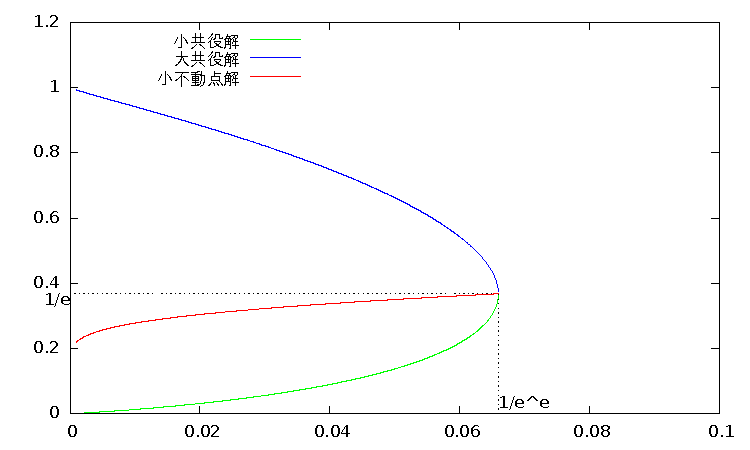
\includegraphics[width=80mm]{../plot/graph/three_roots.pdf}
		\caption{三つの解を持つとき}
		\label{fig:three_roots}
	\end{minipage}
	\end{figure}
	
